\documentclass[UTF8]{ctexart}
\usepackage[colorlinks=true]{hyperref}

\usepackage{amsmath, bm,amsfonts}
\usepackage{hyperref}
\usepackage[normalem]{ulem}
% \usepackage{enumitem}
% \setlist{nosep}
\usepackage{caption}
\usepackage{graphicx}
% \graphicspath{{./pic/}}
\usepackage[usenames, dvipsnames]{xcolor}
\usepackage{color}
\usepackage{listings}
% settings for listings.sty
% \newtheorem{theorem}{\hspace{2em}定理}[Section]
% \newtheorem{theorem}{定理}[section]

\newtheorem{theorem}{\indent 定理}[section]
\newtheorem{lemma}[theorem]{\indent 引理}
\newtheorem{proposition}[theorem]{\indent 命题}
\newtheorem{corollary}[theorem]{\indent 推论}
\newtheorem{definition}{\indent 定义}[section]
\newtheorem{example}{\indent 例}[section]
\newtheorem{remark}{\indent 注}[section]
\newenvironment{solution}{\begin{proof}[\indent\textbf{解}]}{\end{proof}}
\renewcommand{\proofname}{\indent \textbf{证明}}

\renewcommand{\lstlistingname}{代码清单}
\lstdefinestyle{lfonts}{
  basicstyle   = \footnotesize\ttfamily,
  stringstyle  = \color{purple},
  keywordstyle = \color{blue!60!black}\bfseries,
  commentstyle = \color{olive}\scshape,
}
\lstdefinestyle{lnumbers}{
  numbers     = left,
  numberstyle = \tiny,
  numbersep   = 1em,
  firstnumber = 1,
  stepnumber  = 1,
}
\lstdefinestyle{llayout}{
  breaklines       = true,
  tabsize          = 2,
  columns          = flexible,
}
\lstdefinestyle{lgeometry}{
  xleftmargin      = 15pt,
  xrightmargin     = 0pt,
  frame            = tb,
  framesep         = \fboxsep,
  framexleftmargin = 15pt,
}
\lstdefinestyle{lgeneral}{
  style = lfonts,
  style = lnumbers,
  style = llayout,
  style = lgeometry,
}
\def\beginlstdelim#1#2#3{%
  \def\endlstdelim{#2\egroup}%
  \ttfamily#1\bgroup\color{#3}\aftergroup\endlstdelim}
\lstdefinestyle{ldelims}{
  moredelim = **[is][\beginlstdelim{\$}{\$}{orange}]{\$}{\$},
  moredelim = **[is][\beginlstdelim{\{}{\}}{ForestGreen}]{\{}{\}},
  moredelim = **[is][\beginlstdelim{[}{]}{cyan}]{[}{]},
}
% LaTeX lst style
\lstdefinestyle{lltx}{
  language = {[LaTeX]TeX},
  style = lgeneral,
  style = ldelims,
  morekeywords = {% LaTeX original commands
    maketitle,
    rmfamily, sffamily, ttfamily,
    itshape, slshape, scshape,
    mdseries, bfseries, emph,
    textrm, textsf, texttt,
    textit, textsl, textsc,
    textmd, textbf,
    newcommand, renewcommand, providecommand,
    cs, meta, marg, oarg, parg
  }
}
\lstdefinestyle{iltx}{
  style      = lltx,
  basicstyle = \ttfamily
}
\lstdefinestyle{lbash}{
  language   = {bash},
  style      = lgeneral,
}
\lstdefinestyle{ibash}{
  style      = lbash,
  basicstyle = \ttfamily
}

% code style setting
\definecolor{codegreen}{rgb}{0,0.6,0}
\definecolor{codegray}{rgb}{0.5,0.5,0.5}
\definecolor{codepurple}{rgb}{0.58,0,0.82}
\definecolor{backcolour}{rgb}{0.95,0.95,0.92}

\lstdefinestyle{mystyle}{
	backgroundcolor=\color{backcolour},   
	commentstyle=\color{codegreen},
	keywordstyle=\color{magenta},
	numberstyle=\tiny\color{codegray},
	stringstyle=\color{codepurple},
	basicstyle=\footnotesize,
	breakatwhitespace=false,         
	breaklines=true,                 
	captionpos=b,                    
	keepspaces=true,                 
	numbers=left,                    
	numbersep=5pt,                  
	showspaces=false,                
	showstringspaces=false,
	showtabs=false,                  
	tabsize=2
}
\endinput

\usepackage{hologo}
\usepackage{subfigure}
\usepackage{changepage}

\ctexset{
    section = {
        titleformat = \raggedright,
        name = {第,节},
        number = \chinese{section}
    }
}

\title{简易强化学习}
\author{Sisyphes}
% \date{\today}
\date{2020年6月6日}

\begin{document}
\maketitle
\tableofcontents
\newpage

\section{一些废话}

RL的学习应该会比较漫长。一个假想的研究员的学习情况,也许首先会看sutton的 complete draft,
同时实现一些经典算法,然后紧跟学术潮流,看一些来自openAI, DeepMind等的论文,
这中间也许会选一门课程,比如David Silver,伯克利RL或周博磊等,偶尔也许会翻阅一些博客。
我的初略体验(一周)是,这里面会存在一些不可避免的问题,比如流行算法的快速更新,新算法实验成本高,
公式细节上似乎不太严格等。为了较大限度的减少以上问题,扎实经典基础理论,消化新论
文核心思想(不必推导每个细节),加强代码实践,侧重建模能力练习,也许还不错。

本小册子来源于\href{https://github.com/zhoubolei/introRL}{zhoubolei RL},之所以有以上设想,
也源于周老师的讲义,比如在其中会存在(列表可见\ref{sec:seemswrong}),同样的符号,定义有微差
(一些公式来自sutton,一些公式来自新论文,在约定上的细节差异),下标不严谨,期望下标省略,这些会增加一些理解负担,通过做实验来
确定会存在更多其他问题。另外,算法的快速迭代,去推导每一步会显得荒谬,而实际建模有近
似需求,黑盒化,因此着重练习建模能力,在某一具体问题上深入挖掘,或许会不错。周老师的讲课非常棒,提纲挈领,简明扼要,
深入浅出。

所以,本小册子,以基本概念,基本定理,问题建模,代码实现,新论文的近似阅读为逻辑展开。当前版本0.1,将来若有
时间,会逐渐完善。

\newpage
\section{基本认识}
\subsection{什么是强化学习}

\begin{figure}[htbp]
	\centering
	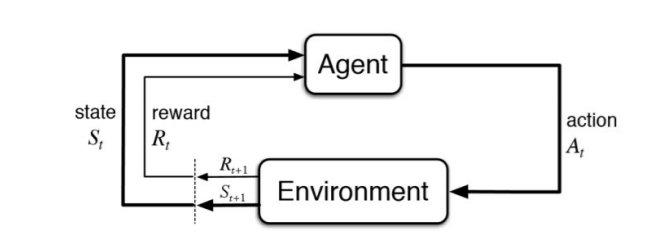
\includegraphics[width=9.7cm, height=3.7cm]{./pic/rl.png}
    \caption{RL Prime}
    \label{subrl1}
\end{figure}
a computational approach to learning whereby an agent tries
to maximize the total amount of reward it receives while
interacting with a complex and uncertain environment. --Sutton and Barto

\begin{itemize}

    \item 基本要素:
    \begin{itemize}
        \item Agent(智能体)
        \item model(模型)
        \item value(价值函数)
        \item policy(策略函数)
    \end{itemize}

    \item 特点:
    \begin{itemize}
        \item 试错探索
        \item 延迟回报
        \item 时间问题(序列数据,无既定分布)
        \item Agent的动作会影响接下来的输入数据,并改变环境的状态
    \end{itemize}
    \item 例子:

    \begin{itemize}
        \item 策略游戏,跑跑卡丁车,纸片游戏,围棋等
        \item 机器人走路,穿衣,抓取东西,拧魔方
        \item 路径规划,机器控制
    \end{itemize}
    
\end{itemize}


\subsection{符号定义}
\subsection{小技巧}
\label{sub:smalltricks}
\textbf{增量平均}:一个简单的变换将序列平均值的计算转化为前一个平均值和当前值与前平均值的“差”的和。
\begin{equation} \label{Incremental:Mean}
    \begin{aligned}
    \mu_{t} &=\frac{1}{t} \sum_{j=1}^{t} x_{j} \\
    &=\frac{1}{t}\left(x_{t}+\sum_{j=1}^{t-1} x_{j}\right) \\
    &=\frac{1}{t}\left(x_{t}+(t-1) \mu_{t-1}\right) \\
    &=\mu_{t-1}+\frac{1}{t}\left(x_{t}-\mu_{t-1}\right)
    \end{aligned} 
\end{equation}

% \tag{label}, amsmath, \label{eqn:einstein}


\textbf{重要采样}:分布$P$不好采样,用更好采样的$Q$替换它,只是需要同时乘以$P$相对于$Q$的权重因子。

\[
E_{x \sim P}[f(x)]=\int f(x) P(x) d x \approx \frac{1}{n} \sum_{i} f\left(x_{i}\right) \label{Important:Sample}
\]

\[
\begin{aligned}
\mathbb{E}_{x \sim P}[f(x)] &=\int P(x) f(x) d x \\
&=\int Q(x) \frac{P(x)}{Q(x)} f(x) d x \\
&=\mathbb{E}_{x \sim Q}\left[\frac{P(x)}{Q(x)} f(x)\right] \approx \frac{1}{n} \sum_{i} \frac{P\left(x_{i}\right)}{Q\left(x_{i}\right)} f\left(x_{i}\right)
\end{aligned}
\]

\textbf{对数求导}:利用对数导数为其倒数的特点,可以将连乘函数的导数和化(注意其和重要采样的联合使用)。

\[
\begin{aligned}
\nabla_{\theta} \mathbb{E}_{x \sim p_{\theta}(x)}[f(x)] &=\nabla_{\theta} \int f(x) p_{\theta}(x) d x \\
&=\int f(x) \nabla_{\theta} p_{\theta}(x) d x \\
&=\int f(x) p_{\theta}(x) \nabla_{\theta} \log p_{\theta}(x) d x \\
&=\mathbb{E}_{x \sim p_{\theta}(x)}\left[f(x) \nabla_{\theta} \log p_{\theta}(x)\right] \\
& \approx \frac{1}{N} \sum_{i=1}^{N} f\left(x_{i}\right) \nabla_{\theta} \log p_{\theta}\left(x_{i}\right)
\end{aligned}
\]


\textbf{重参数化}:利用分布的映射关系,将复杂函数的采样转化为从简单分布采样,然后映射到复杂分布上去,从而达到
解决了复杂分布采样难问题。

\[
\begin{aligned}
\varepsilon & \sim q(\varepsilon) \\
x &=g_{\theta}(\varepsilon) \\
\nabla_{\theta} \mathbb{E}_{x \sim p_{\theta}(x)}[f(x)] &=\nabla_{\theta} \mathbb{E}_{\varepsilon \sim q(\varepsilon)}\left[f\left(g_{\theta}(\varepsilon)\right)\right] \\
&=\mathbb{E}_{\varepsilon \sim q(\varepsilon)}\left[\nabla_{\theta} f\left(g_{\theta}(\varepsilon)\right)\right] \\
& \approx \frac{1}{N} \sum_{i=1}^{N}\left(\nabla_{\theta} f\left(g_{\theta}\left(\varepsilon_{i}\right)\right)\right)
\end{aligned}
\]


\textbf{共轭梯度}:使梯度的方向保持共轭关系(垂直),极大加快优化速度,
\href{https://en.wikipedia.org/wiki/Conjugate_gradient_method}{Conjugate gradient method}


\subsection{基本定理}

\section{Markov Models}
\subsection{MRP}
“\href{https://en.wikipedia.org/wiki/Markov_chain}{Markov chain}因俄国数学家安德烈·马尔可夫得名,
为状态空间中经过从一个状态到另一个状态的转换的随机过程。该过程要求具备“无记忆”的性质:
下一状态的概率分布只能由当前状态决定,在时间序列中它前面的事件均与之无关。”

数学符号语言为:
历史状态:$h_{t}=\left\{s_{1}, s_{2}, s_{3}, \ldots, s_{t}\right\}$,状态$s_t$为Markovian当且仅当
\[ \begin{array}{c}
    p\left(s_{t+1} | s_{t}\right)=p\left(s_{t+1} | h_{t}\right) \\
    p\left(s_{t+1} | s_{t}, a_{t}\right)=p\left(s_{t+1} | h_{t}, a_{t}\right)
    \end{array}
\]

% 容易写出状态转移矩阵
% \[
% P=\left[\begin{array}{cccc}
%     P\left(s_{1} | s_{1}\right) & P\left(s_{2} | s_{1}\right) & \dots & P\left(s_{N} | s_{1}\right) \\
%     P\left(s_{1} | s_{2}\right) & P\left(s_{2} | s_{2}\right) & \dots & P\left(s_{N} | s_{2}\right) \\
%     \vdots & \vdots & \ddots & \vdots \\
%     P\left(s_{1} | s_{N}\right) & P\left(s_{2} | s_{N}\right) & \dots & P\left(s_{N} | s_{N}\right)
%     \end{array}\right]
% \]

若状态转移过程中有奖励(reward),则称之为MRP(Markov Reward Process)。
其基本元素有:
\begin{adjustwidth}{1.3cm}{0cm}
    $S$: 有限状态集($s \in S$)\\
    $P$:状态转移概率$P\left(S_{t+1}=s^{\prime} | s_{t}=s\right)$\\
    $R$:奖励函数(reward)$R\left(s_{t}=s\right)=\mathbb{E}\left[r_{t} | s_{t}=s\right]$\\
    $\gamma$:折扣因子$\gamma \in[0,1]$
\end{adjustwidth}

在实际的RL交互环境中,还需要定义三个变量:

\begin{adjustwidth}{1.3cm}{0cm}
    Horizon: 不同 episode(一个探索周期)的时间步长的最大值\\
    Return: 时间$t$到Horizon的折扣回报和$G_{t}=R_{t+1}+\gamma R_{t+2}+\gamma^{2} R_{t+3}+\gamma^{3} R_{t+4}+\ldots+\gamma^{T-t-1} R_{T} \label{gt}$\\
    状态价值函数:状态$s$在$t$时刻得到的回报的期望值$V_{t}(s)=\mathbb{E}\left[G_{t} | s_{t}=s\right]$
\end{adjustwidth}

根据定义,对价值函数做变换:$V(s)=\mathbb{E}\left[R_{t+1}+\gamma \mathbb{E}\left[R_{t+2}+\gamma R_{t+3}+
\gamma^{2} R_{t+4}+\ldots\right] | s_{t}=s\right]$
容易得出Bellman equation

\begin{equation}
    V(s)=\underbrace{R(s)}_{\text {Immediate reward }}+
    \underbrace{\gamma \sum_{s^{\prime} \in S} P\left(s^{\prime} | s\right) 
    V\left(s^{\prime}\right)}_{\text {Discounted sum of future reward }}
\end{equation}

于是对于有限状态的MRP,有:
$$\begin{array}{c}
    {\left[\begin{array}{c}
    V\left(s_{1}\right) \\
    V\left(s_{2}\right) \\
    \vdots \\
    V\left(s_{N}\right)
    \end{array}\right]=\left[\begin{array}{c}
    R\left(s_{1}\right) \\
    R\left(s_{2}\right) \\
    \vdots \\
    R\left(s_{N}\right)
    \end{array}\right]+\gamma\left[\begin{array}{cccc}
    P\left(s_{1} | s_{1}\right) & P\left(s_{2} | s_{1}\right) & \dots & P\left(s_{N} | s_{1}\right) \\
    P\left(s_{1} | s_{2}\right) & P\left(s_{2} | s_{2}\right) & \dots & P\left(s_{N} | s_{2}\right) \\
    \vdots & \vdots & \ddots & \vdots \\
    P\left(s_{1} | s_{N}\right) & P\left(s_{2} | s_{N}\right) & \dots & P\left(s_{N} | s_{N}\right)
    \end{array}\right]\left[\begin{array}{c}
    V\left(s_{1}\right) \\
    V\left(s_{2}\right) \\
    \vdots \\
    V\left(s_{N}\right)
    \end{array}\right]}
    \end{array}$$

即$V=R+\gamma P V$,其代数解为$V=(I-\gamma P)^{-1} R$。不过实际应用中因$P$过大,
求逆运算复杂度$O\left(N^{3}\right)$过高,会选择迭代方式求解。包含动态规划,蒙特卡洛估计,
Temporal-Difference 学习。

\subsection{MDP}
MDP:在MRP上增加一个动作项,可用$(S, A, P, R, \gamma)$表示。其中
$A$有限的动作集,
$P^{a}, P\left(s_{t+1}=s^{\prime} | s_{t}=s, a_{t}=a\right), 
R\left(s_{t}=s, a_{t}=a\right)=\mathbb{E}\left[r_{t} | s_{t}=s, a_{t}=a\right]$

MDP是对决策过程的建模,目标是在决策集(Policies)中寻找最优决策。其中决策函数是动作在状态空间
的概率分布,用$\pi(a | s)=P\left(a_{t}=a | s_{t}=s\right)$表示状态$s$执行动作$a$的概率,决策
函数是时间独立的,即对任意$t>0$,$A_{t} \sim \pi(a | s)$。

给定MDP($S, A, P, R, \gamma$) 以及决策$\pi$,状态序列$S_1, S_2, \ldots $是一个马尔科夫
过程$(S, P^{\pi})$, 状态、奖励序列$S_1, R_2, S_2, R_3, \ldots$是马尔科夫奖励过程
$(S, P^{\pi}, R^{\pi}, \gamma)$
其中
$$\begin{aligned}
    P^{\pi}\left(s^{\prime} | s\right) &=\sum_{a \in A} \pi(a | s) P\left(s^{\prime} | s, a\right) \\
    R^{\pi}(s) &=\sum_{a \in A} \pi(a | s) R(s, a)
    \end{aligned}
$$


策略$\pi$下开始状态为$s$的状态价值函数
$v^{\pi}(s)=\mathbb{E}_{\pi}\left[G_{t} | s_{t}=s\right]$,
动作价值函数
$q^{\pi}(s, a)=\mathbb{E}_{\pi}\left[G_{t} | s_{t}=s, A_{t}=a\right]$,
表示在状态$s$执行动作$a$后,按照策略$\pi$执行下去的回报期望。
根据以上定义,容易得两者的关系:

\begin{equation}
   v^{\pi}(s)=\sum_{a \in A} \pi(a | s) q^{\pi}(s, a)
\end{equation}

\begin{equation}\label{qsav}
    q^{\pi}(s, a)=R_{s}^{a}+\gamma \sum_{s^{\prime} \in S} P\left(s^{\prime} | s, a\right) v^{\pi}\left(s^{\prime}\right)
\end{equation}


其贝尔曼递归形式也容易写出:
\begin{equation}
v^{\pi}(s)=E_{\pi}\left[R_{t+1}+\gamma v^{\pi}\left(s_{t+1}\right) | s_{t}=s\right]
\end{equation}

\begin{equation}
q^{\pi}(s, a)=E_{\pi}\left[R_{t+1}+\gamma q^{\pi}\left(s_{t+1}, A_{t+1}\right) | s_{t}=s, A_{t}=a\right]
\end{equation}

分别把(4)带入(3),(3)带入(4)得到:
\begin{equation}
    \begin{aligned}
        v^{\pi}(s) &=\sum_{a \in A} \pi(a | s)\left(R(s, a)+\gamma \sum_{s^{\prime} \in S} P\left(s^{\prime} | s, a\right) v^{\pi}\left(s^{\prime}\right)\right)   \\
        q^{\pi}(s, a) &=R(s, a)+\gamma \sum_{s^{\prime} \in S} P\left(s^{\prime} | s, a\right) \sum_{a^{\prime} \in A} \pi\left(a^{\prime} | s^{\prime}\right) 
        q^{\pi}\left(s^{\prime}, a^{\prime}\right) 
    \end{aligned}
\end{equation}


公式(7)的图(Backup Diagram)表示:

\begin{figure}[htbp]
	\centering
	\begin{minipage}[t]{0.48\textwidth}
	\centering
	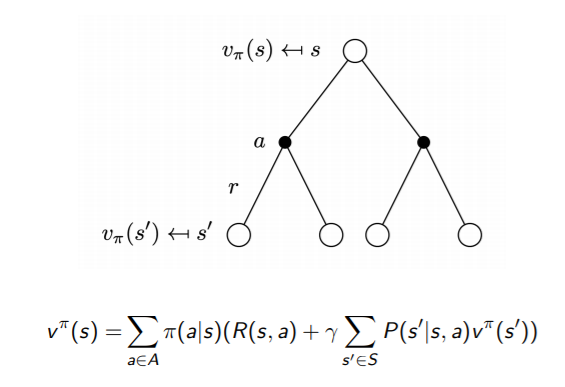
\includegraphics[width=5.5cm, height=3.8cm]{./pic/vpi.png}
	\caption{V}
	\label{piVpi}
	\end{minipage}
	\begin{minipage}[t]{0.48\textwidth}
		\centering
		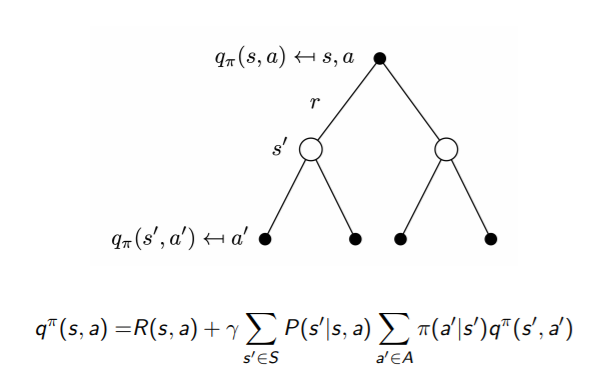
\includegraphics[width=6cm,height=3.7cm]{./pic/qpi.png}
		\caption{Q}
		\label{picQpi}
	\end{minipage}
\end{figure}

简言之,一个状态下可采取不同动作,得到状态动作价值;
一个状态下执行不同的动作,得到奖励,并进入不同的状态;
一个状态并执行了某一动作,得到即刻回报,进入不同状态,并执行不同动作。

建立好模型,并得到了一些关系式,\textbf{问题:如何计算?}

\subsection{评估和优化}

利用\ref{picQpi}, \ref{piVpi}的关系式递推计算,如下迭代:
$$v_{t+1}(s)=\sum_{a \in \mathcal{A}} \pi(a | s)\left(R(s, a)+\gamma \sum_{s^{\prime} 
\in \mathcal{S}} P\left(s^{\prime} | s, a\right) v_{t}\left(s^{\prime}\right)\right),\\
v_{1} \rightarrow v_{2} \rightarrow \ldots \rightarrow v^{\pi}$$
即能得到给定策略$\pi$下的价值函数。
这里递推关系和一般递关系比如Fibonacci数列顺序上
是相反的,在实际优化中会一次更新所有值(有限表格,和关键词bootstrapping吻合),效率虽慢,但能得到最优解。

策略的最优价值函数:$v^{*}(s)=\max _{\pi} v^{\pi}(s)$

最优策略:$\pi^{*}(s)=\arg \max _{\pi} v^{\pi}(s)$
或
$$\pi^{*}(a | s)=\left\{\begin{array}{ll}
    1, & \text { if } a=\arg \max _{a \in A} q^{*}(s, a) \\
    0, & \text { otherwise }
    \end{array}\right.$$

在求得最优状态价值函数或动作价值函数后,根据如上两条定义,很容易得到最优策略。
这个过程被称为值迭代。

这里还有另外一种方式得到最佳策略,一边policy evaluation($V$值更新,划分不是很准确),
一边利用更新的价值函数计算出动作价值函数然后更新策略(greedy)。
即:
$$q^{\pi_{i}}(s, a)=R(s, a)+\gamma \sum_{s^{\prime} \in S} P\left(s^{\prime} | s,
a\right) v^{\pi_{i}}\left(s^{\prime}\right)$$
$$\pi_{i+1}(s)=\underset{a}{\arg \max } q^{\pi_{i}}(s, a)$$

用图可表示为:
\begin{figure}[htbp]
	\centering
	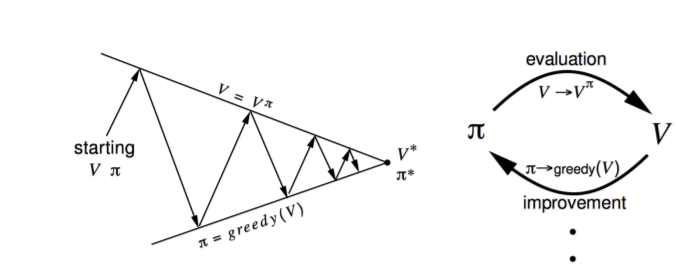
\includegraphics[width=6.7cm, height=2.7cm]{./pic/evalimp.png}
	\caption{rl}
\end{figure}

一个MDP模型存在唯一的最优价值函数(证明见Sutton),但最优策略函数不唯一。


\begin{center}
    Table: Dynamic Programming Algorithms
\end{center}
$$\begin{array}{|c|c|c|}
    \hline \text { Problem } & \text { Bellman Equation } & \text { Algorithm } \\
    \hline \text { Prediction } & \text { Bellman Expectation Equation } & \text { Iterative Policy Evaluation } \\
    \hline \text { Control } & \text { Bellman Expectation Equation } & \text { Policy Iteration } \\
    \hline \text { Control } & \text { Bellman Optimality Equation } & \text { Value Iteration } \\
    \hline
    \end{array}$$

一些存疑的地方:在RL中总是会存在各种分类,这对初学者不太友好。比如上面的总结,以及讲义中给出的
两种策略优化的方式,在第二种方式中为何不直接迭代$Q(s,a)$然后更新策略,以此迭代。另外policy evaluation
是对价值函数$V$的计算,和策略是隐含关系,为何不是值迭代?看上面的表格,就有一点错乱的感觉。中间2,3行是期望
方差,后列对应的却是评估和迭代,而末列3,4行为迭代,对应的中间却一个期望方程,一个最优方程。

简化:值迭代+最后求最值,值迭代+同时策略迭代。

理论补充说明(证明见Sutton):策略优化是一个保序的过程。
一轮优化得到的$\pi^{\prime}(s)=\underset{a}{\arg \max } q^{\pi}(s, a)$有
$v_{\pi^{\prime}}(s) \geq v^{\pi}(s)$,且
\begin{equation}
    \begin{aligned} v^{*}(s) &=\max _{a} q^{*}(s, a) \\ q^{*}(s, a)
        &=R(s, a)+\gamma \sum_{s^{\prime} \in S} P\left(s^{\prime} | s,
        a\right) v^{*}\left(s^{\prime}\right) \end{aligned}
\end{equation}

 于是得到:
 \begin{equation}
    \begin{aligned} v^{*}(s) &=\max _{a} R(s, a)  + \gamma \sum_{s^{\prime} \in S }P\left(s^{\prime} | s,
        a\right) v^{*}\left(s^{\prime}\right)\\ 
        q^{*}(s, a) &=R(s, a)+\gamma \sum_{s^{\prime} \in S} P\left(s^{\prime} | s,
        a\right) \max_{a^{\prime}} q^{*}(s^{\prime}, a^{\prime}) \\
    \end{aligned}
 \end{equation}
 取名为\textbf{最优Bellman方程}。

 以上给出了\ref{subrl1}的MDP建模过程,并给出了在MDP已知的情况下,如何做策略评估,策略迭代,价值迭代。
 但现实世界中MDP模型不存在,或很难给出的情况很常见。
这种情况,可用图\ref{subrl2}来表示。
 \begin{figure}[htbp]
	\centering
	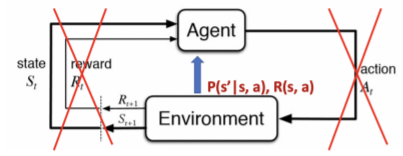
\includegraphics[width=5cm, height=1.6cm]{./pic/rl_free.png}
    \caption{RL Free}
    \label{subrl2}
\end{figure}
学术界称其为Model-free。

\textbf{问题:如何做Model-free 的预测(值估计)和控制(策略优化)?}


\section{Markov Models Free}

Markov Models Free表示没有状态转移和奖励函数的RL模型,如图\ref{subrl2}所示。
此时采用让Agent与环境交互,搜集数据,以频率统计的方式来模拟MDP。于是定义trajectory/episode
$\{S_1, A_1, R_1, S_2, \ldots, S_T, A_T, R_T\}$,表示Agent从状态$S_1$开始做一个完整的(直到结束,terminal)
状态、动作、及时获得的采集链。

那么在策略$\pi$下,如何从利用这些trajectories来评估价值函数?

\subsection{评估(预测)}
对价值函数$V$的估计。
\subsubsection{MC}
$N(s)$表示状态$s$在trajectories出现过的次数(有一次tracjectory表示一次的理解误差),
根据$G_t$定义\eqref{gt},容易从trajectories算出状态$s$下的$G_t$,因$V_t$表示$G_t$的期望,在MC过程,
可用平均值替代,于是结合\eqref{Incremental:Mean},在一个episode/tracjectory中,容易得到
$$\begin{array}{l}
    N\left(S_{t}\right) \leftarrow N\left(S_{t}\right)+1 \\
    v\left(S_{t}\right) \leftarrow v\left(S_{t}\right)+\frac{1}{N\left(S_{t}\right)}\left(G_{t}-v\left(S_{t}\right)\right)
    \end{array}
$$
在不严格要求统计关系的模型中,也可以将其简化为:
$v\left(S_{t}\right) \leftarrow v\left(S_{t}\right)+\alpha \left(G_{t}-v\left(S_{t}\right)\right)$

MC方式的特点:
\begin{itemize}
    \item 必须等到一个episode结束才能更新,从完整的episode中学习
    \item 只能在episodic(terminating,得结束)的环境中学习
    \item 不需要模型具有Markov特性,在非Markov环境中效果更好
\end{itemize}

\subsubsection{TD}
Temporal-Difference Learning,克服了MC的必须实验到状态终结的问题(方差大),
将$G_t$替换为
$R_{t+1} + \gamma v(S_{t+1})$即为$TD(0)$,于是有
\begin{equation}v\left(S_{t}\right) \leftarrow v\left(S_{t}\right)+\alpha\left(R_{t+1}+\gamma v\left(S_{t+1}\right)-v\left(S_{t}\right)\right) \label{TDV} 
\end{equation}
其中$R_{t+1} + \gamma v(S_{t+1})$叫TD target,$\sigma_t=R_{t+1} + \gamma v(S_{t+1})-v(S_t)$叫
TD error。需要注意的是,$v(S_t)$利用了$v(S_{t+1})$,bootstrapping方式,属于自举。

容易想出$TD(\infty)$即为MC。他们的关系可用下图刻画:

\begin{figure}[htbp]
	\centering
	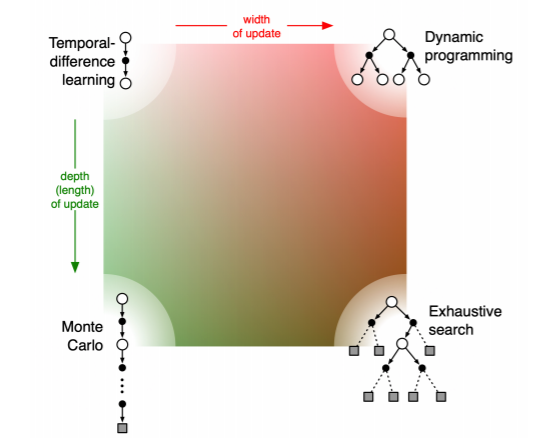
\includegraphics[width=6.4cm, height=5.2cm]{./pic/td_mc_dp_diff.png}
	\caption{mcdptd}
\end{figure}

\subsection{优化(控制)}
策略优化:价值函数迭代+Arg Max或策略迭代(策略估计$Q(s, a)$+策略改进)。

回想上节的策略迭代,是知道$R(s, a), P(s^{\prime}|s, a)$的,但这里未知,如何
在采样的过程中进行策略改进?已有答案是$\epsilon-Greedy$探索法。


$\epsilon-Greedy$ exploration是指以$1-\epsilon$的概率选择使当前动作价值函数
最大的动作,以$\epsilon$的概率选择其余动作,得到新策略:

$$\pi(a | s)=\left\{\begin{array}{ll}
    \epsilon /|\mathcal{A}|+1-\epsilon & \text { if } a^{*}=\arg \max _{a \in \mathcal{A}} Q(s, a) \\
    \epsilon /|\mathcal{A}| & \text { otherwise }
    \end{array}\right.
$$


以这种方式改进策略,有如下定理保证:
\begin{theorem}[Policy improvement theorem]
    For any $\epsilon-greedy$ policy $\pi$, the $\epsilon-greedy$ policy 
    $\pi^{\prime} $with respect $q_{\pi}$ is an improvement, 
    $v_{\pi^{\prime}}(s) \geq v_{\pi}(s)$.
\end{theorem}

证明见Sutton。

于是容易写出$\epsilon-greedy$ 版本的 MC Exploration算法流程:
\begin{figure}[htbp]
	\centering
	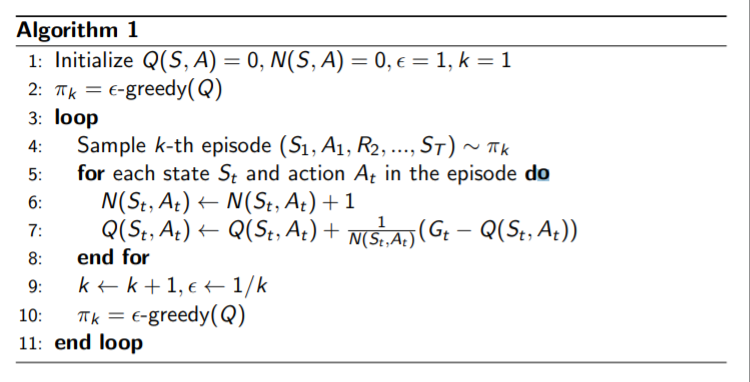
\includegraphics[width=8cm, height=4.1cm]{./pic/mc_epsion.png}
	\caption{mcepsion}
\end{figure}


\subsubsection{Sarsa}
在$\epsilon-greedy$ 策略改进中使用TD而不是MC即为Sarsa算法。
这和在价值更新中将MC改进为TD是同样的道理,且在一定程度上,能减少函数值的方差。
于是容易从\eqref{TDV}中写出$Q(s,a)$函数版本(值估计转化为策略优化)。
$Q\left(S_{t}, A_{t}\right) \leftarrow Q\left(S_{t}, A_{t}\right)+\alpha\left[R_{t+1}+\gamma Q\left(S_{t+1},
 A_{t+1}\right)-Q\left(S_{t}, A_{t}\right)\right]$

综合以上,容易写出one-step 的Sarsa算法流程:

\begin{figure}[htbp]
	\centering
	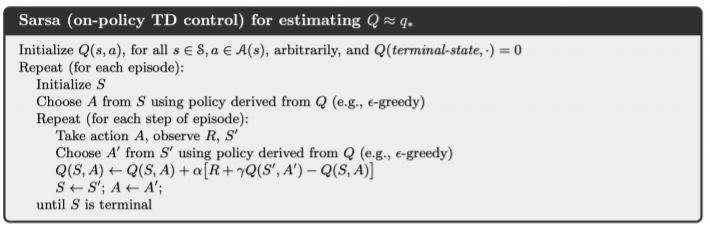
\includegraphics[width=6.1cm, height=2.6cm]{./pic/sarsa.png}
	\caption{sarsa}
\end{figure}

脑补一下n-step版本。

\subsubsection{Q-Learning}
Sarsa明显是自举的(bootstrapping),其在下一步状态所做的动作仍由当前$Q(s,a)$函数选出,
在策略控制上其被分类为On-Policy control,而本小节的Q-Learning为Off-Policy control,其在
下一个状态的动作选择不是由当前$Q$选出。
\begin{equation}\label{qlearning}
    Q\left(S_{t}, A_{t}\right) \leftarrow Q\left(S_{t}, A_{t}\right)+\alpha\left[R_{t+1}+\gamma \max _{a} Q\left(S_{t+1}, a\right)-Q\left(S_{t}, A_{t}\right)\right]
\end{equation}

\subsection{重要采样的应用}
策略$\pi$在优化过程中,其形式可能会变得复杂,不好采样,于是根据\eqref{Important:Sample},
可选择辅助策略$\mu$来生成episodes:$S_{1}, A_{1}, R_{2}, \dots, S_{T} \sim \mu$,
计算其$G_t$。

若Off-Policy 为Monte Carlo,由\eqref{Important:Sample}可得 $G_{told}$和$G_{tnew}$的关系:

$$G_{t}^{\pi / \mu}=\frac{\pi\left(A_{t} | S_{t}\right)}{\mu\left(A_{t} | S_{t}\right)} \frac{\pi\left(A_{t+1} | S_{t+1}\right)}{\mu\left(A_{t+1} | S_{t+1}\right)} \cdots
 \frac{\pi\left(A_{T} | S_{T}\right)}{\mu\left(A_{T} | S_{T}\right)} G_{t}$$

于是在采样策略$\mu$下的其价值更新变为:
$$V\left(S_{t}\right) \leftarrow V\left(S_{t}\right)+\alpha\left(G_{t}^{\pi / \mu}-V\left(S_{t}\right)\right)$$

若Off-Policy为TD,容易得到其价值更新为:
\begin{equation}
    V\left(S_{t}\right) \leftarrow V\left(S_{t}\right)+\alpha\left(\frac{\pi\left(A_{t} | S_{t}\right)}{\mu\left(A_{t} | S_{t}\right)}\left(R_{t+1}+
\lambda V\left(S_{t+1}\right)\right)-V\left(S_{t}\right)\right)
\end{equation}


\textbf{问题:离线策略Q-Learning为何不能使用重要采样?}

因为Q-Learning不需要在策略分布上做价值的期望估计。
完整答案请看
\href{https://www.quora.com/Why-doesn-t-DQN-use-importance-sampling-Dont-we-always-use-this-method-to-correct-the-sampling-error-produced-by-the-off-policy}{这里}。

\subsection{DP和TD的差异}

$$\begin{array}{l|l}
    \text { Expected Update (DP) } & \text { Sample Update (TD) } \\
    \hline \text { Iterative Policy Evaluation } & \text { TD Learning } \\
    V(s) \leftarrow \mathbb{E}\left[R+\gamma V\left(S^{\prime}\right) | s\right] & V(S) \leftarrow^{\alpha} R+\gamma V\left(S^{\prime}\right) \\
    \hline \text { Q-Policy Iteration } & \text { Sarsa } \\
    Q(S, A) \leftarrow \mathbb{E}\left[R+\gamma Q\left(S^{\prime}, A^{\prime}\right) | s, a\right] & Q(S, A) \leftarrow^{\alpha} R+\gamma Q\left(S^{\prime}, A^{\prime}\right) \\
    \hline \text { Q-Value Iteration } & \text { Q-Learning } \\
    Q(S, A) \leftarrow \mathbb{E}\left[R+\gamma \max _{a^{\prime} \in \mathcal{A}} Q\left(S^{\prime}, A^{\prime}\right) | s, a\right] & Q(S, A) \leftarrow^{\alpha} R+\gamma \max _{a^{\prime} \in \mathcal{A}} Q\left(S^{\prime}, a^{\prime}\right) \\
    \hline \text { where } x \leftarrow^{\alpha} y \text { is defined as } x \leftarrow x+\alpha(y-x) & \\
 \end{array}
 $$

\section{函数参数化}
前面提出的一些值估计,策略改进的方法,但都是以统计为基础,在和环境交互的同时,搜集状态
序列,计算统计量,进行价值,状态动作函数的更新(表格式计算)。经典的例子Cliff walk:$4\times 16$个状态;Mountain car:1600个状态;
Tic-Tac-Toe:1000个状态。但当面对西洋棋($10^{47}$),围棋($10^{170}$),器械臂、直升机(连续状态)等情况,
就显得肌无力。使用带参数的函数,优化参数是可行的。数学上可表达如下:

\begin{equation}
    \begin{aligned}
    \hat{v}(s, \mathbf{w}) & \approx v^{\pi}(s) \\
    \hat{q}(s, a, \mathbf{w}) & \approx q^{\pi}(s, a) \\
    \hat{\pi}(a, s, \mathbf{w}) & \approx \pi(a | s)
    \end{aligned}
\end{equation}
这样做还有另一个好处,有了关于状态的具体函数,可计算所有状态的价值。

\textbf{问题:怎么具体设计函数?参数如何更新?策略如何优化?}
本小节回答前两问,第三问见节\ref{sec:PGD}(当采用可微函数时)。

\begin{figure}[htbp]
	\centering
	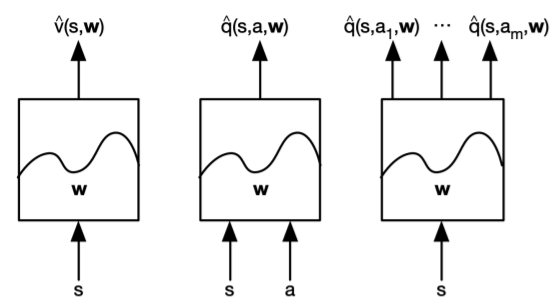
\includegraphics[width=5.1cm, height=3.2cm]{./pic/func_design.png}
    \caption{func design}
    \label{func:design}
\end{figure}

函数逼近的可选方案:
\begin{itemize}
    \item 特征的线性组合
    \item 神经网络
    \item 决策树
    \item 最邻距离
\end{itemize}
这里只关心可微方式,输入输出参考\ref{func:design}。

\subsection{线性组合}

对于特征的线性组合,若用$\mathbf{x}(s)=\left(x_{1}(s), \ldots, x_{n}(s)\right)^{T}$
表示状态特征向量,则价值函数可表示为:$\hat{v}(s, \mathbf{w})=\mathbf{x}(s)^{T} \mathbf{w}=\sum_{j=1}^{n} x_{j}(s) w_{j}$,
若目标函数采用平方差,则优化目标:$J(\mathbf{w})=\mathbb{E}_{\pi}\left[\left(v^{\pi}(s)-\mathbf{x}(s)^{T} \mathbf{w}\right)^{2}\right]$
其梯度更新:$\Delta \mathbf{w}=\alpha\left(v^{\pi}(s)-\hat{v}(s, \mathbf{w})\right) \mathbf{x}(s)$
,若把参数更新方式写成文字形式,有:

$$\textbf{参数变化量} = \textbf{步长} \times \textbf{预测误差} \times \textbf{特征向量}$$

数学抽象做完了,回到实际环境中,需要把理想的$v^{\pi}(s)$替换回实际中的值。结合上一节的MC,TD
更新方式,容易得到各自对应的更新版本。

对MC: 
$\Delta \mathbf{w}=\alpha\left(G_{t}-\hat{v}(s_t, \mathbf{w})\right) \nabla_{\mathbf{w}} \hat{v}\left(s_{t}, \mathbf{w}\right)$

对TD(0):
$\Delta \mathbf{w}=\alpha\left(R_{t+1} + \gamma \hat{v}(s_{t+1}, \mathbf{w})-\hat{v}(s_t, \mathbf{w})\right) \nabla_{\mathbf{w}} \hat{v}\left(s_{t}, \mathbf{w}\right)$

在线性组合的方式下,

MC:
$\Delta \mathbf{w}=\alpha\left(G_{t}-\hat{v}(s_t, \mathbf{w})\right) \mathbf{x}(s_t)$

TD(0):
$\Delta \mathbf{w}=\alpha\left(R_{t+1} + \gamma \hat{v}(s_{t+1}, \mathbf{w})-\hat{v}(s_t, \mathbf{w})\right)  \mathbf{x}(s_t)$

需要注意的是,上述梯度下降为semi-gradient,因为其目标值中它自己。

同理可得,控制算法的更新方式:

MC:
\begin{equation}\Delta \mathbf{w}=\alpha\left(G_{t}-\hat{q}\left(s_{t}, a_{t}, \mathbf{w}\right)\right) \nabla_{\mathbf{w}} \hat{q}\left(s_{t}, a_{t}, \mathbf{w}\right)\end{equation}

Sarsa:
\begin{equation}\Delta \mathbf{w}=\alpha\left(R_{t+1}+\gamma \hat{q}\left(s_{t+1}, a_{t+1}, \mathbf{w}\right)-\hat{q}\left(s_{t}, a_{t}, \mathbf{w}\right)\right) \nabla_{\mathbf{w}} \hat{q}\left(s_{t}, a_{t}, \mathbf{w}\right)\end{equation}

Q-Learning:
\begin{equation}\Delta \mathbf{w}=\alpha\left(R_{t+1}+\gamma \max _{a} \hat{q}\left(s_{t+1}, a, \mathbf{w}\right)-\hat{q}\left(s_{t}, a_{t}, \mathbf{w}\right)\right) \nabla_{\mathbf{w}} \hat{q}\left(s_{t}, a_{t}, \mathbf{w}\right)\end{equation}
Sarsa的VFA(Value Function Approximation)控制算法流程:

\begin{figure}[htbp]
	\centering
	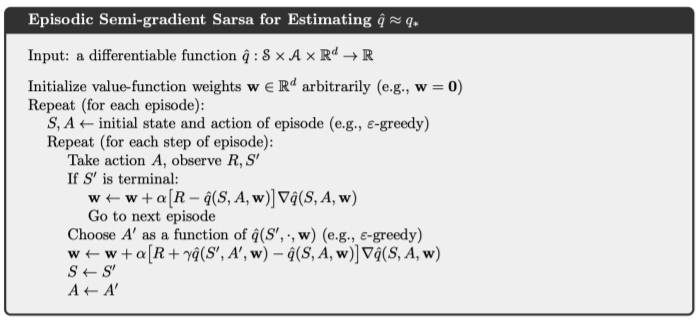
\includegraphics[width=7.1cm, height=3.5cm]{./pic/sarsa_vfa.png}
    \caption{sarsa vfa}
    \label{sarsa:vfa}
\end{figure}

\textbf{问题:参数逼近的控制算法收敛性如何?}见下表:

\begin{figure}[htbp]
	\centering
	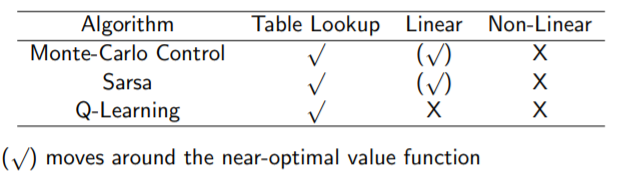
\includegraphics[width=8.1cm, height=2.8cm]{./pic/converge_vfa.png}
    \caption{converge vfa}
    \label{converge:vfa}
\end{figure}


\subsection{DQN}
特征线性组合的难点和以前CV手工设计特征类似,如何做出好的特征表示,如何对复杂问题进行有效的特征选取等问题。
类似于CNN替换SIFT,ORB等特征提取方式,2015年,DeepMind发表了一篇名为“Human-level control through deep reinforcement learning”
的文章,将DL引入了RL,给出了一种有效的价值函数的非线性表达方法,同时不需要手工设计特征,并在
Breakout, Pong, Montezuma’s Revenge, Private Eye四款游戏上达到了人类专家水平。随之而来的是DQN的各种升级,可参考
\href{https://deepmind.com/blog/article/Agent57-Outperforming-the-human-Atari-benchmark}{DQN综述}。

DQN对Atari Games的建模\ref{DQN:Atari},
\begin{figure}[htbp]
	\centering
	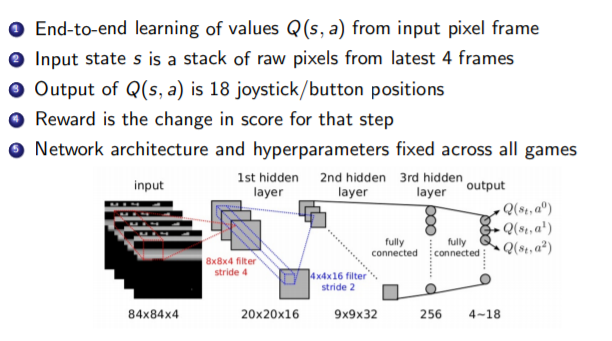
\includegraphics[width=6.7cm, height=3.7cm]{./pic/DQN_Atari.png}
    \caption{DQN Atari}
    \label{DQN:Atari}
\end{figure}
从中可以看到基本思想就是:输入像素图,输出状态动作函数值。该建模方式有一些固有的坑,
论文中对采样关联,目标值非平稳两个问题给出了解决方案,分别是经验池采样,固定目标函数。

经验池是指设定一个缓存区$\mathcal{D}$, 存放历史样本
$\left(s, a, r, s^{\prime}\right)$,并从中采样。
固定目标函数是指,使用另外一组参数$\mathbf{w}^{-}$来计算目标值$r+\gamma \max _{a^{\prime}} \hat{Q}(s^{\prime}, a^{\prime}, \mathbf{w}^{-})$,
这里样本来自$\mathcal{D}$。
最终参数更新量为:
\begin{equation}
    \Delta \mathbf{w}=\alpha\left(r+\gamma \max _{a^{\prime}} \hat{Q}\left(s^{\prime}, a^{\prime}, \mathbf{w}\right)-
Q(s, a, \mathbf{w})\right) \nabla_{\mathbf{w}} \hat{Q}(s, a, \mathbf{w})
\end{equation}

% DQN的问题远不止以上两点,综述论文可参考:\href{https://arxiv.org/pdf/1710.02298.pdf}{Rainbow}
\section{策略参数化}
\subsection{基础建模}
\label{sec:PGD}
上一节提出了函数参数化,并给出了值函数的实现例子,这一节给出策略函数的实现方式。虽然arg max 值函数可得到策略,
但这种方式基本不能给出随机策略,实际情况,会有大量非完全确定的策略需求,比如在石头剪刀布游戏中,其最优策略(纳什均衡点)为随机策略,
在一些带有闭环的探索游戏中,也需要随机策略来避免无限循环。而若将策略函数设置为动作的概率分布函数,则可实现这一点,同时有也可省去
值函数。

设$\pi_{\theta}(s, a)$是以$\theta$为参数的策略函数,如何定义策略的质量?

在episodic环境中,可定义为:$J_{1}(\theta)=V^{\pi_{\theta}}(s_1)=\mathbb{E}_{\pi_{\theta}}[v_1]$,
始状态的期望价值。在持续(continuing)环境中,可以有两种定义方式:利用平均价值有,$J_{avV}(\theta)=\sum_{s}d^{\pi_{\theta}}(s)V^{\pi_{\theta}}(s)$,
利用一步时间段的平均回报值有,$J_{avR}(\theta)=\sum_{s}d^{\pi_{\theta}}(s)\sum_{a}\pi_{\theta}(s,a)R(s,a)$,
其中$d^{\pi_{\theta}}$是$\pi_{\theta}$的马尔科夫平稳分布。直观来讲,最后一种更为方便,其对应优化目标可表示为:

\begin{equation}\theta^{*}=\underset{\theta}{\arg \max } \mathbb{E}_{\tau \sim \pi_{\theta}}
\left[\sum_{t} r\left(s_{t}, a_{t}^{\tau}\right)\right]\end{equation}
其中$\tau$是策略函数$\pi_{\theta}$下的一个采样trajectory。

对于$J(\theta)$的优化:若$J(\theta)$可微,可用梯度下降,共轭梯度,拟-牛顿等方法,若$J(\theta)$不可微,或倒数难算,可用采用
Cross-entropy method (CEM),Hill climbing,Evolution algorithm等。


在多步MDP模型中,状态-动作 trajectory服从以下关系:
$$\tau = (s_0, a_0, r_1, 
\ldots, s_{T-1}, r_{T-1}, s_T) \sim (\pi_{\theta},
P(s_{t+1}|s_{t}, a_t)),$$
用$R_{\tau}=\sum_{t=0}^{T}R(s_t, a_t)$表示一trajector的回报和。于是
\begin{equation}\label{mdpjthta} J(\theta)=\mathbb{E}_{\pi_{\theta}}\left[\sum_{t=0}^{T} R\left(s_{t}, 
a_{t}\right)\right]=\sum_{\tau} P(\tau ; \theta) R(\tau),\end{equation}
其中$P(\tau ; \theta)=\mu\left(s_{0}\right) \prod_{t=0}^{T-1} \pi_{\theta}\left(a_{t} | s_{t}\right) p\left(s_{t+1} | s_{t}, a_{t}\right)$
表示策略$\pi_{\theta}$下,该trajectory出现的概率。此时优化目标为:

\begin{equation}\theta^{*}=\underset{\theta}{\arg \max } J(\theta)=
\underset{\theta}{\arg \max } \sum_{\tau} P(\tau ; \theta) R(\tau)\end{equation}
结合\ref{sub:smalltricks}的对数技巧,容易得出式\eqref{mdpjthta}的梯度为:

\begin{equation}\nabla_{\theta} J(\theta)=\sum_{\tau} P(\tau ; \theta) R(\tau) \nabla_{\theta} \log P(\tau ; \theta)\end{equation}
将$\nabla_{\theta} \log P(\tau ; \theta)$展开:
\begin{equation}\begin{aligned}
    \nabla_{\theta} \log P(\tau ; \theta) &=\nabla_{\theta} \log \left[\mu\left(s_{0}\right) \prod_{t=0}^{T-1} \pi_{\theta}\left(a_{t} | s_{t}\right) p\left(s_{t+1} | s_{t}, a_{t}\right)\right] \\
    &=\nabla_{\theta}\left[\log \mu\left(s_{0}\right)+\sum_{t=0}^{T-1} \log \pi_{\theta}\left(a_{t} | s_{t}\right)+\log p\left(s_{t+1} | s_{t}, a_{t}\right)\right] \\
    &=\sum_{t=0}^{T-1} \nabla_{\theta} \log \pi_{\theta}\left(a_{t} | s_{t}\right)
    \end{aligned}
\end{equation}
于是多步MDP的策略梯度最终表示为:
\begin{equation}
\nabla_{\theta} J(\theta) \approx \frac{1}{m} \sum_{i=1}^{m} R\left(\tau_{i}\right) \sum_{t=0}^{T-1} \nabla_{\theta} 
\log \pi_{\theta}\left(a_{t}^{i} | s_{t}^{i}\right)
\end{equation}

最终的梯度公式可以做一个直观认识:{\color{red}对于权重函数的期望(积分),其梯度方向为原始概率的对数的导数乘以对应权重(注意这里是一个trajectory)}。
有了这一直观认识,我们可以猜一猜其他各种形式的策略优化函数的梯度。

当权重值为$G_t$(在一个trajectory,从时间t开始获得的奖励)时:
\begin{equation} \label{JGt} \nabla_{\theta} J(\theta)=\mathbb{E}_{\pi_{\theta}}\left[\sum_{t=0}^{T-1} G_{t} 
    \cdot \nabla_{\theta} \log \pi_{\theta}\left(a_{t} | s_{t}\right)\right]\end{equation}

当权重值为$Q_{w}(s_t, a_t)$时:
\begin{equation} \label{JQsa}\nabla_{\theta} J(\theta)=\mathbb{E}_{\pi_{\theta}}\left[\sum_{t=0}^{T-1} Q_{\color{red}{w}}(s_t, a_t)
    \cdot \nabla_{\color{red}{\theta}} \log \pi_{\theta}\left(a_{t} | s_{t}\right)\right]\end{equation}

验证:见周博磊讲义第5章。也就是说以上猜测确为事实。

不过在一个trajectory中,$G_t$往往方差较大,如何做到减小其方差,但保持其期望不变?
答案是减去回报值的期望。

基准值$b(s_t) = \mathbb{E}[r_t + r_{t+1} + \ldots + r_{T-1}]$,有
$\mathbb{E}_{\tau}[\nabla_{\theta}\log\pi_{\theta}(a_{t}|s_t)b(s_t))]=0$,并且
\begin{equation}\begin{aligned}
    E_{\tau}\left[\nabla_{\theta} \log \pi_{\theta}\left(a_{t} | s_{t}\right)\left(G_{t}-b\left(s_{t}\right)\right)\right] &=E_{\tau}\left[\nabla_{\theta} \log \pi_{\theta}\left(a_{t} | s_{t}\right) G_{t}\right] \\
    \operatorname{Var}_{\tau}\left[\nabla_{\theta} \log \pi_{\theta}\left(a_{t} | s_{t}\right)\left(G_{t}-b\left(s_{t}\right)\right)\right] &<\operatorname{Var}_{\tau}\left[\nabla_{\theta} \log \pi_{\theta}\left(a_{t} | s_{t}\right) G_{t}\right]
    \end{aligned}
\end{equation}

于是优化函数变为:
\begin{equation} \label{JGt} \nabla_{\theta} J(\theta)=\mathbb{E}_{\pi_{\theta}}\left[\sum_{t=0}^{T-1} {\color{red} (G_{t} - b_{w}(s_t))}
\cdot \nabla_{\theta} \log \pi_{\theta}\left(a_{t} | s_{t}\right)\right]\end{equation}

如法炮制,\eqref{JQsa}也可做减基准值的改动。不过这里还是回到RL原始的发展顺序来。在教材中,\eqref{JQsa}被称为
Actor-Critic Policy Gradient,原因在于$Q_{w}(s, a)$担任了Actor的角色,$\pi_{\theta}(a|s)$扮演了
Critic角色,他们各自有各自的参数,这和生成模型GAN异曲同工。

\subsubsection{演员评论家}
当用线性价值函数来逼近Actor时:$Q_{\mathbf{w}}(s,a)=\phi(s, a)^{T}\mathbf{w}$。
此时Critic由线性的$TD(0)$更新,Actor由策略梯度更新。一个简单版本见\ref{QAC}。

\begin{figure}[htbp]
	\centering
	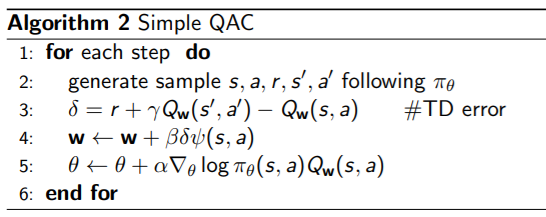
\includegraphics[width=8cm, height=3.1cm]{./pic/QAC.png}
    \caption{QAC}
    \label{QAC}
\end{figure}

上面提到的Actor-Critic算法的减基改动,怎么做?回想一下策略$\pi$下的$Q,V$的定义是什么。
$Q^{\pi, \gamma}(s, a)=\mathbb{E}_{\pi}\left[r_{1}+\gamma r_{2}+\ldots | s_{1}=s, a_{1}=a\right]$

$V^{\pi, \gamma}(s)=\mathbb{E}_{\pi}\left[r_{1}+\gamma r_{2}+\ldots | s_{1}=s\right]=\mathbb{E}_{a \sim \pi}[Q^{\pi, \gamma}(s,a)]$
因状态价值函数是状态-动作价值函数的无偏估计,因此,只需做$Q \leftarrow Q -V$(按算法更新写法)即可。
于是我们得到一个重要的函数:优势函数。
\begin{definition}[Advantage function]
    $$A^{\pi, \gamma}(s, a) = Q^{\pi, \gamma}(s, a) - V^{\pi, \gamma}(s) $$
\end{definition}

其对对应的策略梯度为:

\begin{equation} \label{JAC}  \begin{aligned}\nabla_{\theta} J(\theta)&=\mathbb{E}_{\pi_{\theta}}\left[\sum_{t=0}^{T-1} (Q_{{\color{red} w}}(s_t, a_t) - V(s_t))
\cdot \nabla_{\theta} \log \pi_{{\color{red} \theta}}\left(a_{t} | s_{t}\right)\right] \\
&= \mathbb{E}_{\pi_{\theta}}\left[\sum_{t=0}^{T-1} (A_{{\color{red} w}}(s_t, a_t)
\cdot \nabla_{\theta} \log \pi_{{\color{red} \theta}}\left(a_{t} | s_{t}\right)\right] \end{aligned}
\end{equation}

以上就是基本的策略梯度算法。那么策略梯度有什么问题?我想应该需要更详细的推导,分析,以及实验了。
关于策略梯度能克服不可微操作,可参考\href{http://karpathy.github.io/2016/05/31/rl/}{PG overcome the non-differentiable computation}。

\subsection{策略梯度的改进}
不同算法的优缺点,除了理论推导,实际实验情况也非常重要。
\subsubsection{Policy Gradient→TRPO→ACKTR→PPO}

在\href{https://arxiv.org/abs/1506.02438}{High-Dimensional Continuous Control Using Generalized Advantage Estimation}一文中,
可以看到,策略梯度可以有多种:
\begin{equation}\begin{aligned}
    \nabla_{\theta} J(\theta) &=\mathbb{E}_{\pi_{\theta}}\left[\nabla_{\theta} \log \pi_{\theta}(s, a) G_{t}\right]-\text { REINFORCE } \\
    &=\mathbb{E}_{\pi_{\theta}}\left[\nabla_{\theta} \log \pi_{\theta}(s, a) Q^{\mathrm{w}}(s, a)\right]-\mathrm{Q} \text { Actor-Critic } \\
    &=\mathbb{E}_{\pi_{\theta}}\left[\nabla_{\theta} \log \pi_{\theta}(s, a) A^{\mathrm{w}}(s, a)\right]-\text { Advantage Actor-Critic } \\
    &=\mathbb{E}_{\pi_{\theta}}\left[\nabla_{\theta} \log \pi_{\theta}(s, a) \delta\right]-\text { TD Actor-Critic }
    \end{aligned}
\end{equation}
前三种已经见过了,对于第四种,其和优势函数的关系,可能并不能一眼看出。
其实我们有如下结论:
\begin{corollary}
    设价值函数,$TD$ 误差分别为$V^{\pi_{\theta}(s)}$, $\delta^{\pi_{\theta}}=r(s, a)+\gamma V^{\pi_{\theta}}\left(s^{\prime}\right)-V^{\pi_{\theta}}(s)$,则
    $\mathbb{E}_{\pi_{\theta}}[\delta^{\pi_{\theta}}|s,a] = A^{\pi_{\theta}}(s,a)$。
\end{corollary}
根据\eqref{qsav},即可证明。

策略梯度的问题:
\begin{itemize}
    \item 因为在线学习的原因,采样效率不高
    \item 策略更新过大或者步长不合理会导致训练崩溃
    \begin{itemize}
        \item 和强监督不同这里更新的数据不是独立的
        \item 步长太大,导致策略不好,不好的策略搜集了更差的数据,恶性循环严重
        \item 很难从坏策略中逃出来,大概率致使模型崩塌
    \end{itemize}
\end{itemize}

\begin{figure}[htbp]
	\centering
	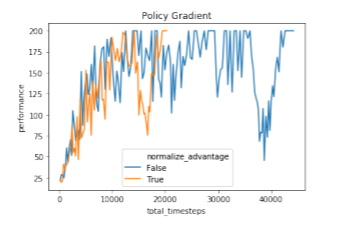
\includegraphics[width=5.6cm, height=3.4cm]{./pic/traning_stable.png}
    \caption{traning unstatble}
    \label{traning:unstatble}
\end{figure}

为了解决训练不稳定,在线更新问题,John Schulman等人在TRPO中提出了用置信区间和自然梯度
下降来克服训练不稳定问题,并顺势而为,用重要采样将在线改为离线。

核心思想就是限制策略更新前后的差异。因为策略是概率函数,于是可用KL散度来
限制。$$d^{*}=\arg \max J(\theta+d), \text { s.t. } K L\left[\pi_{\theta} \| \pi_{\theta+d}\right]=c$$
将重要采样用上则为:
$$\begin{array}{l}
    \qquad J_{\theta_{\text {old }}}(\theta)=\mathbb{E}_{t}\left[\frac{\pi_{\theta}\left(a_{t} | s_{t}\right)}{\pi_{\theta_{\text {old }}}\left(a_{t} | s_{t}\right)} R_{t}\right] \\
    \text { subject to } K L\left(\pi_{\theta_{\text {old }}}\left(. | s_{t}\right)|| \pi_{\theta}\left(. | s_{t}\right)\right) \leq \delta
    \end{array}
$$
经过一些计算,得到更新方式:
$$\theta_{t+1}=\theta_{t}+\sqrt{\frac{2 \delta}{g^{T} H^{-1} g}} H^{-1} g$$
其中
$$H=\nabla_{\theta}^{2} K L\left(\pi_{\theta_{t}} \| \pi_{\theta}\right)=E_{a, s \sim \pi_{\theta_{t}}}\left[\nabla_{\theta} \log \pi_{\theta}(a, s) \nabla_{\theta} \log \pi_{\theta}(a, s)^{T}\right]$$

综合以上,TRPO算法的自然梯度下降算法流程:

\begin{figure}[htbp]
	\centering
	\begin{minipage}[t]{0.48\textwidth}
	\centering
	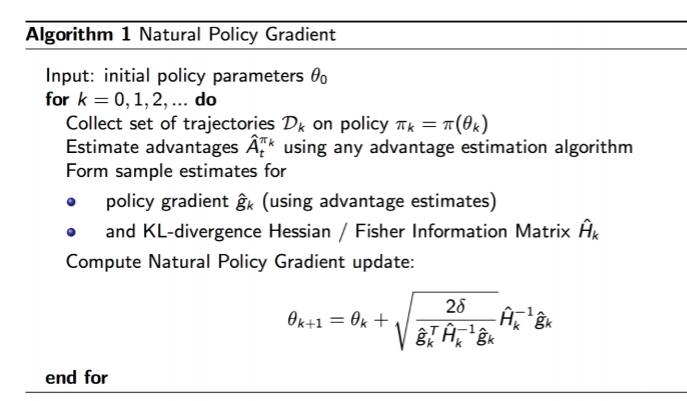
\includegraphics[width=6.8cm, height=4.2cm]{./pic/TRPO.png}
    \caption{Nature TRPO}
    \label{Nature:TRPO}
	\end{minipage}
	\begin{minipage}[t]{0.48\textwidth}
		\centering
        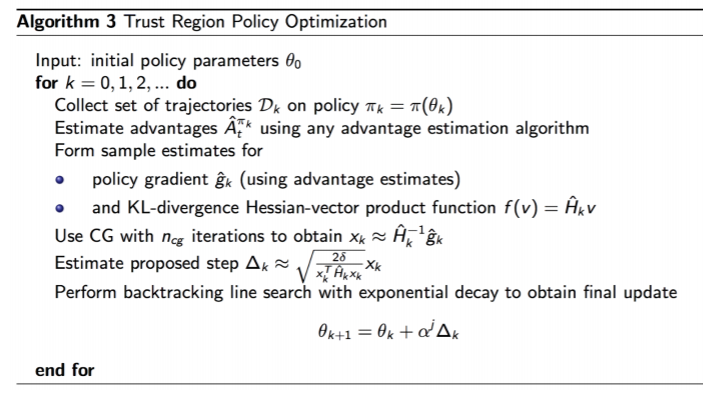
\includegraphics[width=7cm, height=4cm]{./pic/TRPO_2.png}
        \caption{Conjugate Nature TRPO}
        \label{Nature:CTRPO}
	\end{minipage}
\end{figure}

将Fisher Information Matrix的逆用共轭算法实现的算法流程见\ref{Nature:CTRPO}。


而ACKTR则对FIM的逆的计算做了进一步改进(使用了矩阵的分块计算)。


PPO做了两点改进,第一将合并了TRPO的限制条件和函数主体:
$$\operatorname{maximize}_{\theta} \mathbb{E}_{t}\left[\frac{\pi_{\theta}\left(a_{t} | 
s_{t}\right)}{\pi_{\theta_{\text {old }}}\left(a_{t} | s_{t}\right)} A_{t}\right]-\beta
 \mathbb{E}_{t}\left[K L\left[\pi_{\theta_{\text {old }}}\left(\cdot | s_{t}\right),
  \pi_{\theta}\left(\cdot | s_{t}\right)\right]\right]$$
合并的好处是省略了二阶导数的计算,完全转化为一阶导数,时间上更快。

在前后策略差异的限制上,$\delta$也做了动态调整,见\ref{PPO:Penalty}。

第二对新旧策略和优势函数上做了一些简单粗暴的限制。具体如下:

$$L_{t}(\theta)=\min \left(r_{t}(\theta) \hat{A}_{t}, \operatorname{clip}\left(r_{t}(\theta), 1-\epsilon, 1+\epsilon\right) \hat{A}_{t}\right)$$
直观上理解,当新旧策略的比率在($1-\epsilon, 1+\epsilon$)之外时,优势函数将按如上截取。
也就是说要当新旧策略差距大时,对策略函数做惩罚。

算法流程如下:

\begin{figure}[htbp]
	\centering
	\begin{minipage}[t]{0.48\textwidth}
	\centering
    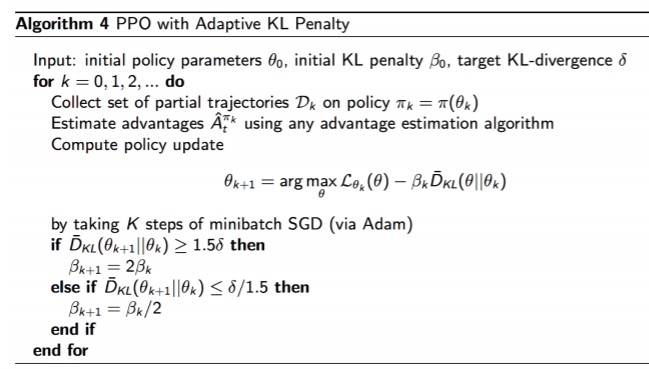
\includegraphics[width=6.5cm, height=3.7cm]{./pic/PPO_KL.png}
    \caption{PPO KL Penalty}
    \label{PPO:Penalty}
	\end{minipage}
	\begin{minipage}[t]{0.48\textwidth}
		\centering
        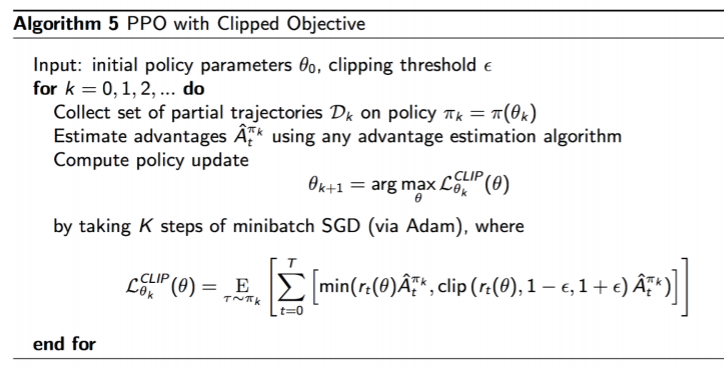
\includegraphics[width=6.2cm, height=3.7cm]{./pic/PPO_Clip.png}
        \caption{PPO Clip}
        \label{PPO:Clip}
	\end{minipage}
\end{figure}


\subsubsection{Q-learning→DDPG→TD3→SAC}
DDPG为DQN的连续版本。

\section{Model Based}

\section{模仿学习}

\section{分布式系统}
后续也许着重了解。

\section{Code}
算法基本都有开源实现,环境模拟有
\href{https://gym.openai.com/}{gym},\href{http://www.mujoco.org/}{MojoCO}等。

\href{https://github.com/higgsfield/RL-Adventure-2}{RL-Adventure-2}:干净简洁明的实现了DQN+PG系列;
\href{https://github.com/sfujim/TD3/}{TD3}:论文细节完备实现;
\href{https://github.com/cuhkrlcourse/DeepRL-Tutorials}{DeepRL-Tutorials Codes}:RL-Adventure的复杂版本。

Code目录代码选自RL-Adventure-2。
% \begin{lstlisting}[python]
    
% \end{lstlisting}

\section{可能都是我错了}
\label{sec:seemswrong}
\begin{itemize}
    \item 章节3,p11,$(S_1, A_1, R_1, \ldots, S_t)$的$R_1$是之前的$R_2$写法不一致,一个是及时奖励,一个是奖励函数的延迟奖励?
    \item 第3章,p20,$G_{t}^{(1)}=R_{t+1}+\gamma v(S_{t+1})$这里的$v(S_t)$和原始的$V(S_t)$意思似乎不太一致,在
    Sutton书中p143,是定义的形式,此处在头上加了(1),效果也看成定义,但原始的$V$是$G$的期望,正常来说折扣和和状态是有关的。
    % 若$G_{t}^{(1)}$理解成当前状态的期望回报,就能说通了,但这不就是原始$V_t$吗。
    \item 第3章,p33的等式开头是不是错了?Sutton的也如此。
    \item 第5章,p13,$r(s_t, a_{t}^{\tau})$不是折扣和,但p12却用了$R(s, a)$,这和以前的符号,似乎矛盾。
    \item 第5章,p19的3 Likelihood ratios,似乎和维基上的不太一致。具体含义可参考\href{http://blog.shakirm.com/2015/11/machine-learning-trick-of-the-day-5-log-derivative-trick/}{log LR}
    \item 第5章,p23$R_{\tau}$对应了$(T+1)$个$R(s_t, a_t)$,应该改为$T-1$?
    \item 第5章,p27$V$应该是$J$。
    \item 第6章,p20,21$KL$在new, old上面似乎不一致。
\end{itemize}
\end{document}